
% v2-acmsmall-sample.tex, dated March 6 2012
% This is a sample file for ACM small trim journals
%
% Compilation using 'acmsmall.cls' - version 1.3 (March 2012), Aptara Inc.
% (c) 2010 Association for Computing Machinery (ACM)
%
% Questions/Suggestions/Feedback should be addressed to => "acmtexsupport@aptaracorp.com".
% Users can also go through the FAQs available on the journal's submission webpage.
%
% Steps to compile: latex, bibtex, latex latex
%
% For tracking purposes => this is v1.3 - March 2012
\documentclass[prodmode,acmtecs]{acmsmall} % Aptara syntax
\usepackage[spanish,polish]{babel}
\usepackage[T1]{fontenc}
\usepackage{fancyvrb}
\usepackage{graphicx,hyperref}
\newcommand\cutout[1]{}


\usepackage[table]{xcolor}
\usepackage[utf8]{inputenc}
\usepackage[parfill]{parskip}
\usepackage{tabulary}
\PassOptionsToPackage{hyphens}{url}
\usepackage{hyperref}    
\usepackage[capitalize]{cleveref}


% Metadata Information
% !!! TODO: SET THESE VALUES !!!
\acmVolume{0}
\acmNumber{0}
\acmArticle{CFP}
\acmYear{0}
\acmMonth{0}

\newcounter{colstart}
\setcounter{page}{4}

\RecustomVerbatimCommand{\VerbatimInput}{VerbatimInput}%
{
%fontsize=\footnotesize,
fontfamily=\rmdefault
}


\newcommand{\UnderscoreCommands}{%\do\verbatiminput%
\do\citeNP \do\citeA \do\citeANP \do\citeN \do\shortcite%
\do\shortciteNP \do\shortciteA \do\shortciteANP \do\shortciteN%
\do\citeyear \do\citeyearNP%
}

\usepackage[strings]{underscore}



% Document starts
\begin{document}


\setcounter{colstart}{\thepage}

\acmArticle{CFP}
\title{\huge\sc SIGLOG Monthly 224}
\author{DAVID PURSER\affil{University of Warsaw, Poland}
\vspace*{-2.6cm}\begin{flushright}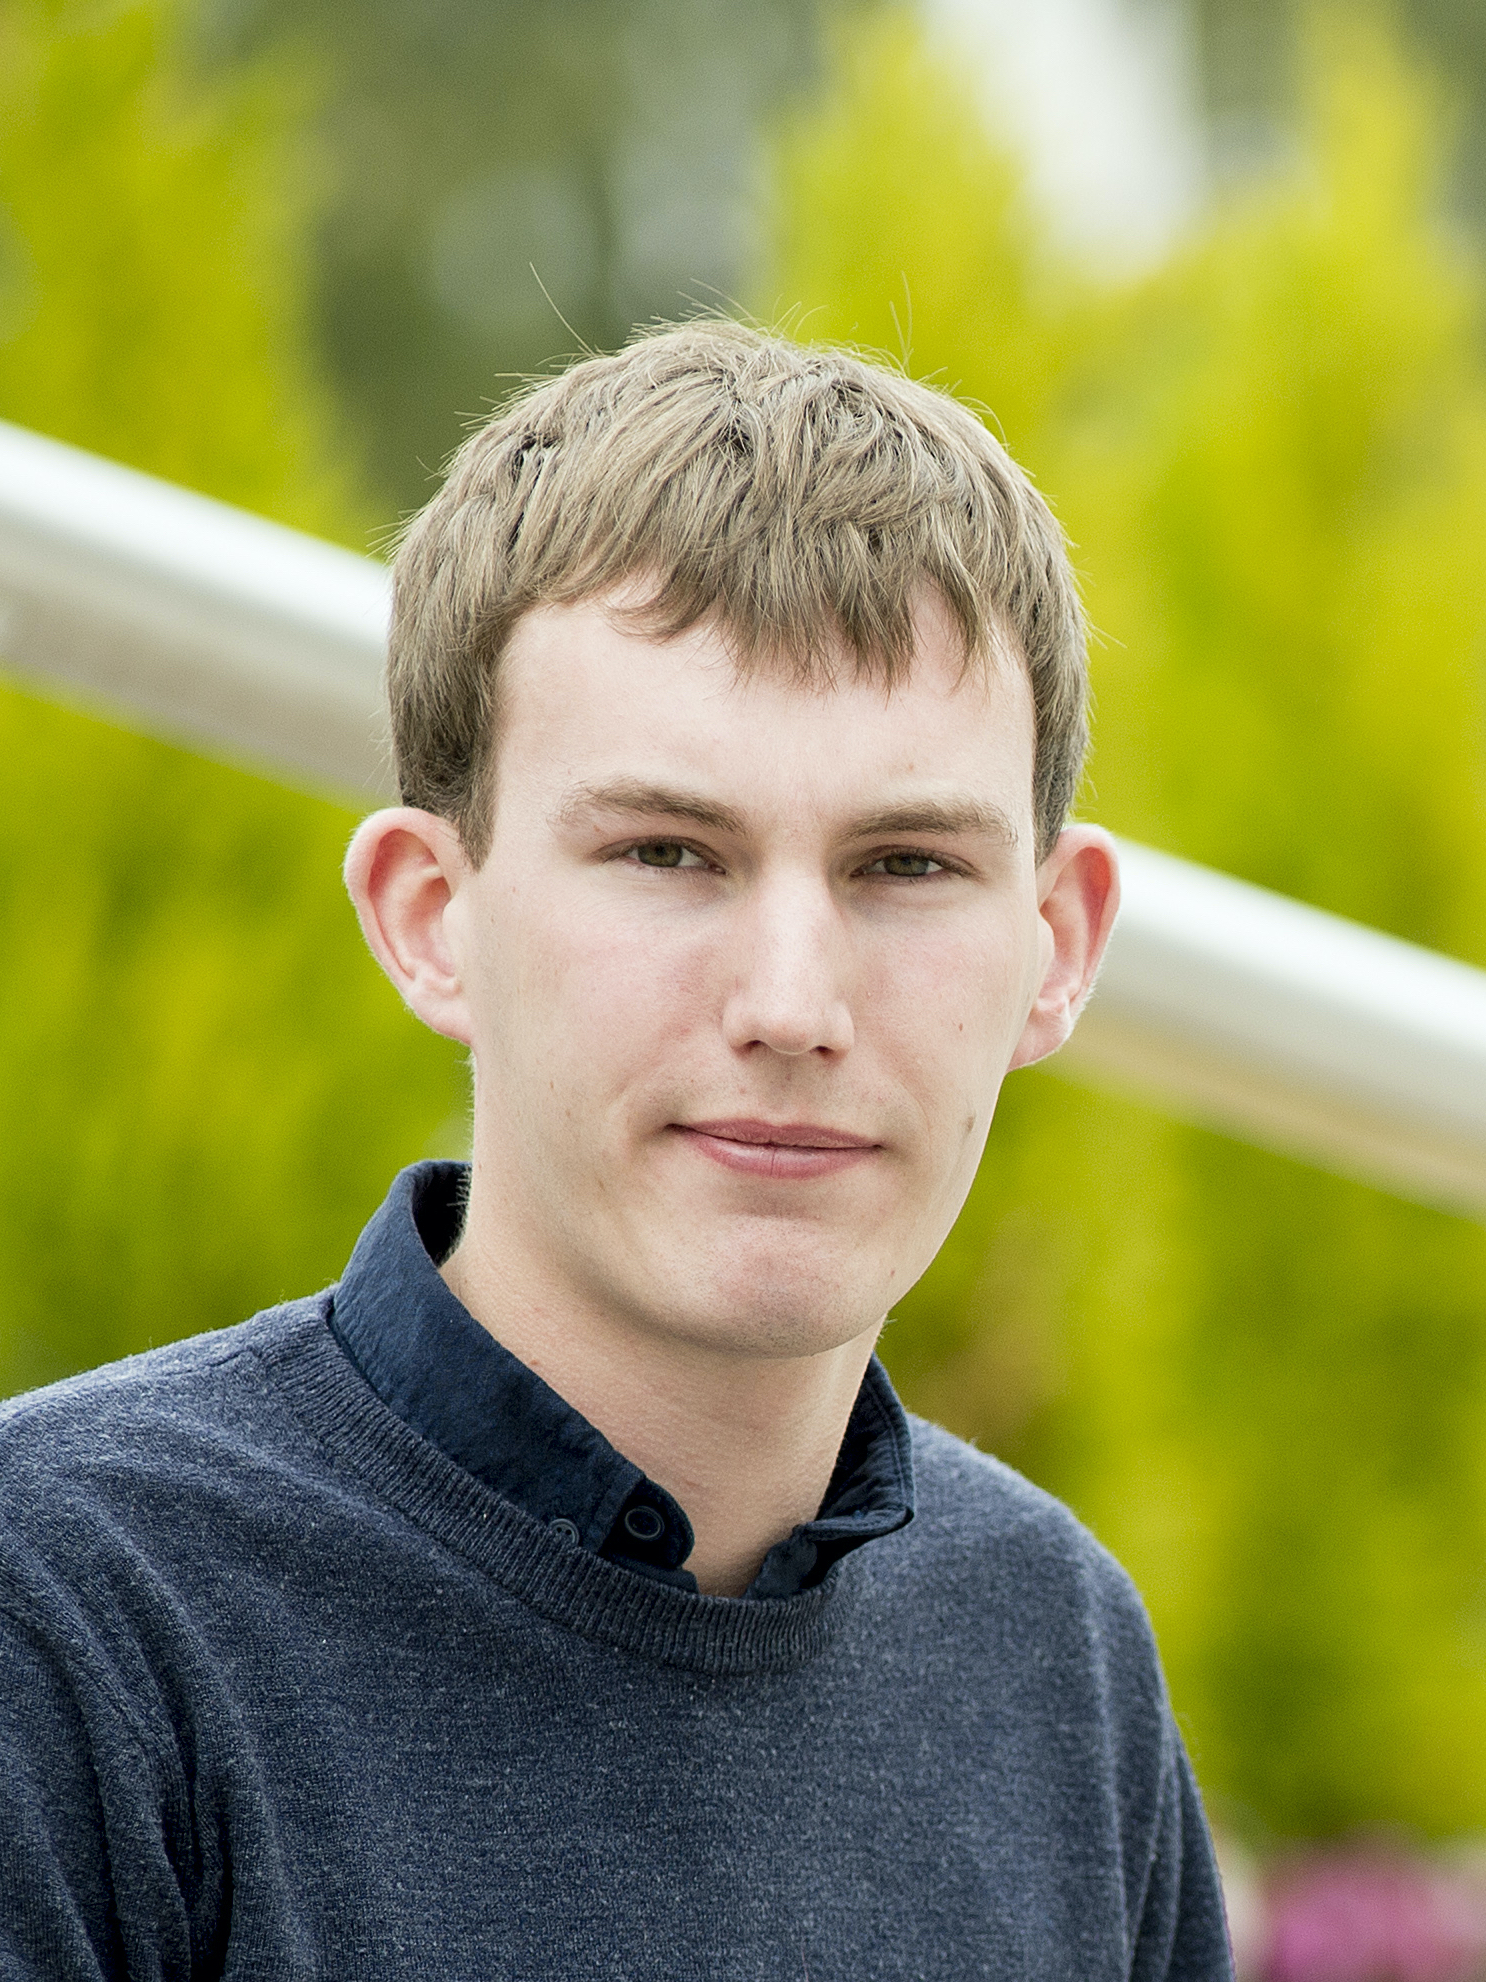
\includegraphics[width=30mm]{dp}\end{flushright}
}

\maketitlee

\href{https://lics.siglog.org/newsletters/}{Past Issues}
 - 
\href{https://lics.siglog.org/newsletters/inst.html}{How to submit an announcement}
\section{Table of Content}\begin{itemize}\item DEADLINES (\cref{deadlines}) 
 
\item CALLS 
 
\begin{itemize}\item Alonzo Church Award (CALL FOR NOMINATIONS) (\cref{AlonzoChurchAward})
\item FLoC'22 MW (CALL FOR APPLICATIONS FOR TRAVEL SCHOLARSHIP) (\cref{FLoC22MW})
\item E. W. Beth Outstanding Dissertation Prize 2022 (CALL FOR NOMINATIONS) (\cref{EWBethOutstandingDissertationPrize2022})
\item IWC 2022 (CALL FOR PAPERS) (\cref{IWC2022})
\item WPTE 2022 (CALL FOR PAPERS) (\cref{WPTE2022})
\item Algorithmic Law Design and Implementation (CALL FOR PARTICIPATION) (\cref{AlgorithmicLawDesignandImplementation})
\item Eleventh Summer School on Formal Techniques (CALL FOR PARTICIPATION) (\cref{EleventhSummerSchoolonFormalTechniques})
\item Runtime Verification 2022 (CALL FOR PAPERS) (\cref{RuntimeVerification2022})
\item LogTeach-22 (CALL FOR PAPERS) (\cref{LogTeach22})
\item ASL 2022 (CALL FOR PAPERS) (\cref{ASL2022})
\item LAMAS\&SR 2022 (CALL FOR CONTRIBUTIONS) (\cref{LAMASSR2022})
\item GandALF 2022 (CALL FOR PAPERS) (\cref{GandALF2022})
\item FSCD 2024 (CALL FOR LOCATION) (\cref{FSCD2024})
\item Datalog 2.0 2022 (CALL FOR PAPERS) (\cref{Datalog202022})
\end{itemize} 
\item JOB ANNOUNCEMENTS 
 
\begin{itemize}\item PhD student position on proof theory and verification of legal software (\cref{PhDstudentpositiononprooftheoryandverificationoflegalsoftware})
\item 10 PhD Positions at TU Wien (\cref{10PhDPositionsatTUWien})
\end{itemize} 
\end{itemize}\section{Deadlines}\label{deadlines}\rowcolors{1}{white}{gray!25}\begin{tabulary}{\linewidth}{LL}Alonzo Church Award:  & Apr 02, 2022 (Deadline for nominations) \\
PhD student position on proof theory and verification of legal software:  & Apr 03, 2022 (Deadline) \\
LearnAut:  & April 07, 2022 (Submission deadline, EXTENDED) \\
FLoC'22 MW:  & Apr 11, 2022 (Deadline for applications) \\
NALOMA 22:  & Apr 15, 2022 (Papers \& extended abstracts) \\
E. W. Beth Outstanding Dissertation Prize 2022:  & Apr 15, 2022 (Deadline for nominations) \\
FORMATS 2022:  & Apr 19, 2022 (Abstract), Apr 22, 2022 (Paper) \\
GCM 2022:  & Apr 20, 2022 (Abstract Submission), Apr 27, 2022 (Paper Submission) \\
DECFOML:  & Apr 22, 2022 (Submissions) \\
LPNMR 2022:  & Apr 23, 2022 (Paper registration), Apr 30, 2022 (Paper) \\
WPTE 2022:  & Apr 26, 2022 (Abstract), May 03, 2022 (Paper) \\
10 PhD Positions at TU Wien:  & Apr 30, 2022 (Deadline 1st Call) \\
ATVA 2022:  & May 01, 2022 (Abstract, extended), May 08, 2022 (Paper, extended) \\
MOVEP2022:  & May 01, 2022 (Student Abstract), Apr 30, 2022 (Early registration deadline) \\
IWC 2022:  & May 02, 2022 (Paper) \\
Runtime Verification 2022:  & May 05, 2022 (Paper) \\
ASL 2022:  & May 10, 2022 (Papers), May 10, 2022 (Papers due) \\
NSV 2022:  & May 10, 2022 (Paper) \\
LogTeach-22:  & May 10, 2022 (Abstract), May 20, 2022 (Paper) \\
LAMAS\&SR 2022:  & May 23, 2022 (Paper) \\
PODS 2023:  & May 30, 2022 (First cycle abstract), Jun 06, 2022 (Full paper), Nov 28, 2022 (Second cycle abstract), Dec 05, 2022 (Full paper) \\
FSCD 2024:  & Jun 27, 2022 (Deadline for proposals) \\
ACKERMANN AWARD 2022:  & Jul 01, 2022 (Deadline for nomination) \\
Datalog 2.0 2022:  & Jul 01, 2022 (Paper registration), Jul 08, 2022 (Paper) \\
\end{tabulary}
\section{Alonzo Church Award:}\label{AlonzoChurchAward}CALL FOR NOMINATIONS 

\begin{itemize}\item  SIGLOG reminds you to submit nominations for the Alonzo Church Award by April 02, 2022. 
 
\end{itemize}\section{FLoC'22 MW: FLoC 2022 Mentoring Workshop}\label{FLoC22MW}  \href{https://www.floc2022.org/flocmentoringworkshop}{https://www.floc2022.org/flocmentoringworkshop}\\ 
  1 August 2022 and 5 August 2022\\ 
  Haifa, Israel\\ 
CALL FOR APPLICATIONS FOR TRAVEL SCHOLARSHIP 

\begin{itemize}\item  We warmly invite students to apply for travel scholarships to attend the Mentoring Workshop and FLoC.  The deadline for applications is April 11th. Applications are received via the form at \href{https://forms.gle/QxWmYcvQCPgXRxEq6}{https://forms.gle/QxWmYcvQCPgXRxEq6} 
 
Deadline for applications: Apr 11, 2022 
 
\item  ABOUT THE MENTORING WORKSHOP 
 
  The purpose of the FLoC 2022 Mentoring Workshop (FLoC'22 MW) is to provide mentoring and career advice to early-stage graduate students, to attract them to pursue research careers in various logic-related areas. The workshop will particularly encourage participation of women and under-represented minorities. 
 
  There will be two workshop days, one for each FLoC Conference Block, so the students can choose which one of the two they prefer to attend. The workshop program will include a number of talks and interactive sessions. The talks will give an overview of the field along with brief introductions to the varied topics highlighted at FLoC. Other talks will provide mentoring and career advice, from academia and industry. 
 
\item  CONFIRMED SPEAKERS 
 
  Mentoring Workshop for FLoC Conference Block 1 (Friday, August 5th, 2022)  
 
\begin{itemize}\item  TBA (check the website for updates!)
\end{itemize} 
  Mentoring Workshop for FLoC Conference Block 2 (Friday, August 5th, 2022) 
 
\begin{itemize}\item  Rajeev Alur, University of Pennsylvania, USA
\item  Kristin Rozier, Iowa State University, USA
\item  Natarajan Shankar, SRI, USA
\item  Alexandra Silva, Cornell University, USA
\end{itemize} 
\end{itemize}\section{E. W. Beth Outstanding Dissertation Prize 2022:}\label{EWBethOutstandingDissertationPrize2022}CALL FOR NOMINATIONS 

\begin{itemize}\item  ABOUT 
 
  Since 1998, the Association for Logic, Language, and Information (FoLLI) has been awarding the annual E.W. Beth Dissertation Prize to outstanding Ph.D. dissertations in Logic, Language, and Information (\href{http://www.folli.info/?page_id=74}{http://www.folli.info/?page\_id=74}), with financial support of the E.W. Beth Foundation (\href{https://www.knaw.nl/en/awards/funds/evert-willem-beth-stichting/evert-willem-beth-foundation}{https://www.knaw.nl/en/awards/funds/evert-willem-beth-stichting/evert-willem-beth-foundation}).  
 
  In accordance with the aim of the Beth Foundation to continue and extend the work of the Dutch logician Evert Willem Beth, nominations are invited of outstanding dissertations on topics in the broad remit of ESSLLI, in logic, language, information and computation. Interdisciplinary dissertations with results impacting various of these research areas in their investigations are especially solicited. Nominations are now invited for outstanding dissertations in these areas resulting in a Ph.D. degree awarded in 2021.  
 
Deadline for nominations: Apr 15, 2022 
 
\item  Qualifications: 
 
\begin{itemize}\item  A Ph.D. dissertation on a related topic is eligible for the Beth Dissertation Prize 2022, if the degree was awarded between January 1st and December 31st, 2021.
\item  There are no restrictions on the nationality, ethnicity, age, gender or employment status of the author of the nominated dissertation, nor on the university, academic department or scientific institution formally conferring the Ph.D. degree, nor on the language in which the dissertation has originally been written.
\item  If a nominated dissertation has originally been written in a language other than English, its file should still contain the required 10 page English abstract, see below. If the committee decides that a nominated dissertation in a language other than English requires translation to English for proper evaluation, the committee can transfer its nomination to the competition in 2023. The English translation must in such cases be submitted before the deadline of the call for nominations in 2023. The committee may recommend the Beth Foundation to consider supporting such nominated dissertations for English translation, upon request by the author of the dissertation. 
\end{itemize} 
\item  The prize consists of:  
 
\begin{itemize}\item  a certificate
\item  a donation of 3000 euros, provided by the E.W. Beth Foundation, divided among the winners, should there be more than one winner
\item  an invitation to submit the dissertation, possibly after revision, for publication in FoLLI Publications on Logic, Language and Information (Springer). 
\end{itemize} 
 Only digital submissions are accepted, without exception. Hard copy submissions are not allowed. The following documents are to be submitted in a single nomination file in zip format:  
 
\begin{itemize}\item  The original dissertation in pdf format (ps/doc/rtf etc. not acceptable).
\item  A ten-page English abstract of the dissertation, presenting the main results of each chapter.
\item  A letter of nomination from the dissertation supervisor, which concisely describes the scope and significance of the dissertation, stating when the degree was officially awarded and the members of the Ph.D. committee. Nominations should contain the address, phone and email details of the nominator.
\item  Two additional letters of support, including at least one from a referee not affiliated with the academic institution that awarded the Ph.D. degree, nor otherwise related to the nominee (e.g. former teachers, supervisors, co-authors, publishers or relatives) or the dissertation.
\item  Self-nominations are not possible. 
\end{itemize} 
  All pdf documents must be submitted electronically, as one zip file, via EasyChair by following the link \href{https://easychair.org/conferences/?conf=bodp2022}{https://easychair.org/conferences/?conf=bodp2022}. In case of any problems or questions please contact the chair of the committee Mehrnoosh Sadrzadeh (m.sadrzadeh@ucl.ac.uk).  
 
  The prize will be awarded by the chair of the FoLLI board at a ceremony during the 33rd ESSLLI summer school, in Galway, August 8-19, 2021.  
 
\end{itemize}\section{IWC 2022: 11th International Workshop on Confluence}\label{IWC2022}  1st August 2022, Haifa, Israel\\ 
  Affiliated with FSCD @ FLoC 2022\\ 
  \href{http://cl-informatik.uibk.ac.at/iwc/2022/}{http://cl-informatik.uibk.ac.at/iwc/2022/}\\ 
CALL FOR PAPERS 

\begin{itemize}\item  BACKGROUND 
 
  Confluence provides a general notion of determinism and has been conceived as one of the central properties of rewriting systems. Confluence relates to many topics of rewriting (completion, modularity, termination, commutation, etc.) and has been investigated in many formalisms of rewriting, such as first-order rewriting, lambda-calculi, higher-order rewriting, constraint rewriting, conditional rewriting, and so on. Recently there is a renewed interest in confluence research, resulting in new techniques, tool support, confluence competition, and certification as well as in new applications. The scope of the workshop is all these aspects of confluence and related topics. 
 
  The goal of the workshop is to provide a forum for researchers interested in the topic of confluence to exchange and share new developments in the field. The workshop will enable discussion on theoretical results, new problems, applications, implementations and benchmarks, and share the current state-of-the-art on the development of confluence tools. 
 
  The 11th Confluence Competition CoCo 2022 will run live during IWC 2022. 
 
\item  Topics 
 
\begin{itemize}\item  confluence and related properties (unique normal forms, commutation, ground confluence)
\item  completion
\item  critical pair criteria
\item  decidability issues
\item  complexity issues
\item  system descriptions
\item  certification
\item  applications of confluence 
\end{itemize} 
\item  IMPORTANT DATES (AoE) 
 
\rowcolors{1}{white}{gray!25}\begin{tabulary}{\linewidth}{LL}Paper submission:  & May 02, 2022 \\
notification:  & Jun 05, 2022 \\
workshop:  & Aug 01, 2022 \\
\end{tabulary}
 
\item  SUBMISSION 
 
  We solicit short papers or extended abstracts of at most five pages. There will be no formal reviewing. In particular, we welcome short versions of recently published articles and papers submitted elsewhere. The program committee checks relevance and may provide additional feedback. The accepted papers will be made available electronically before the workshop. 
 
  The page limit for papers is 5 pages in EasyChair style.  
 
\end{itemize}\section{WPTE 2022: 9th International Workshop on Rewriting Techniques for Program Transformations and Evaluation}\label{WPTE2022}  July 31, 2022\\ 
  \href{https://wpte2022.github.io/}{https://wpte2022.github.io/}\\ 
  \href{https://easychair.org/conferences/?conf=wpte2022}{https://easychair.org/conferences/?conf=wpte2022}\\ 
CALL FOR PAPERS 

\begin{itemize}\item  New! Publication will be organised for selected papers as part of a Special Issue in the Journal of Logical and Algebraic Methods in Programming. 
 
\item  The aim of WPTE is to bring together the researchers working on program transformations, evaluation, and operationally based programming language semantics, using rewriting methods, in order to share the techniques and recent developments and to exchange ideas to encourage further activation of research in this area. 
 
\item  TOPICS 
 
\begin{itemize}\item  Correctness of program transformations, optimizations and translations.
\item  Program transformations for proving termination, confluence, and other properties.
\item  Correctness of evaluation strategies.
\item  Operational semantics of programs, operationally-based program equivalences such as contextual equivalences and bisimulations.
\item  Cost-models for arguing about the optimizing power of transformations and the costs of evaluation.
\item  Program transformations for verification and theorem proving purposes.
\item  Translation, simulation, equivalence of programs with different formalisms, and evaluation strategies.
\item  Program transformations for applying rewriting techniques to programs in specific programming languages.
\item  Program transformations for program inversions and program synthesis.
\item  Program transformation and evaluation for Haskell and rewriting.
\end{itemize} 
\item  IMPORTANT DATES (AoE) 
 
\rowcolors{1}{white}{gray!25}\begin{tabulary}{\linewidth}{LL}Abstract submission:  & Apr 26, 2022 \\
Paper submission:  & May 03, 2022 \\
Notifications:  & Jun 15, 2022 \\
Final version for informal proceedings:  & Jun 29, 2022 \\
Workshop:  & Jul 31, 2022 \\
Post-proceedings (JLAMP special issue):  & autumn 2022 \\
\end{tabulary}
 
\end{itemize}\section{Algorithmic Law Design and Implementation: }\label{AlgorithmicLawDesignandImplementation}  April 28-29, 2022 Barcelona\\ 
CALL FOR PARTICIPATION 

\begin{itemize}\item  About 
 
  From April 28 — April 29, 2022, we will hold the in-situ Conference on Algorithmic Law Design and Implementation in Barcelona.  This is a highly interdisciplinary event with speakers and attendees among different communities like logicians, computer scientists, practicing lawyers, public administrators, industrial professionals, and legal scholars. 
 
  An important logical aspect of the conference is how formal verification techniques (both proof assistants and model checking) can be set to work to prevent errors in critical legal software and to warrant legal principles as fairness, accountability and transparency. Various related technical, juridical, philosophical, and practical aspects will be discussed during the conference.  
 
\item  Registration and more information can be found at: \href{https://www.ub.edu/prooftheory/event/lawdesign/}{https://www.ub.edu/prooftheory/event/lawdesign/} 
 
\end{itemize}\section{Eleventh Summer School on Formal Techniques:}\label{EleventhSummerSchoolonFormalTechniques}  May 30 - June 5, 2022, Menlo College, Atherton, California\\ 
  \href{http://fm.csl.sri.com/SSFT22}{http://fm.csl.sri.com/SSFT22}\\ 
CALL FOR PARTICIPATION 

\begin{itemize}\item  The Eleventh Summer School on Formal Techniques is directed at graduate students and young researchers. A prior background in formal methods is helpful but not required. This year, the school will take place in a hybrid mode: the lectures and labs will be live-streamed and recorded, but we strongly encourage in-person participation. Funding for transportation/food/lodging is available for US-based students. 
 
\item  The lecturers at the school include Corina Pasareanu (NASA Ames/CMU West), Randy Bryant (CMU), Sanjit Seshia (UC Berkeley), Ruzica Piskac (Yale University), and Mayur Naik (U. of Pennsylvania). 
 
\item  We also have distinguished invited talks from Thomas Wies (New York University), Phokion G. Kolaitis (University of California Santa Cruz and IBM Research), Maria Paola Bonacina (Università degli Studi di Verona), Susmit Jha (SRI International) 
 
\item  The main lectures in the summer school start on Tuesday May 31 and will be preceded by a background course on logic given by Natarajan Shankar (SRI) and Stephane Graham-Lengrand (SRI) on Monday May 30 and a mini-bootcamp on Sunday June 5. 
 
Registration deadline: Apr 30, 2022 
 
\end{itemize}\section{Runtime Verification 2022:}\label{RuntimeVerification2022}  \href{https://rv22.gitlab.io}{https://rv22.gitlab.io}\\ 
CALL FOR PAPERS 

\begin{itemize}\item  We are pleased to invite you to submit papers for the 22nd International Conference on Runtime Verification (RV'22), which will take place as part of the Computational Logic Autumn Summit CLAS 2022 (\href{http://viam.science.tsu.ge/clas2022/}{http://viam.science.tsu.ge/clas2022/}) in Tbilisi, Georgia, from September 28-30, 2022. 
 
\item  DATES (AoE) 
 
\rowcolors{1}{white}{gray!25}\begin{tabulary}{\linewidth}{LL}Paper submission:  & May 05, 2022 \\
Notification:  & Jun 22, 2022 \\
Camera-ready:  & Jul 24, 2022 \\
Conference:  & Sep 28-30, 2022 \\
\end{tabulary}
 
\item  Conference Objectives and Scope  
 
  Runtime verification is concerned with the monitoring and analysis of the runtime behaviour of software and hardware systems. Runtime verification techniques are crucial for system correctness, reliability, and robustness; they provide an additional level of rigor and effectiveness compared to conventional testing and are generally more practical than exhaustive formal verification. Runtime verification can be used prior to deployment, for testing, verification, and debugging purposes, and after deployment for ensuring reliability, safety, and security and for providing fault containment and recovery as well as online system repair. 
 
\item  TOPICS 
 
  The topics of the conference include, but are not limited to: 
 
\begin{itemize}\item  specification languages for monitoring
\item  monitor construction techniques
\item  program instrumentation
\item  logging, recording, and replay
\item  combination of static and dynamic analysis
\item  specification mining and machine learning over runtime traces
\item  monitoring techniques for concurrent and distributed systems
\item  runtime checking of privacy and security policies
\item  metrics and statistical information gathering
\item  program/system execution visualization
\item  fault localization, containment, resilience, recovery and repair
\item  systems with learning-enabled components
\item  dynamic type checking and assurance cases
\item  runtime verification for autonomy and runtime assurance
\end{itemize} 
  Application areas of runtime verification include cyber-physical systems, autonomous systems, safety/mission critical systems, enterprise and systems software, cloud systems, reactive control systems, health management and diagnosis systems, and system security and privacy. 
 
\item  PAPERS  
 
  There are four categories of papers which can be submitted: regular, short, tool demo, and benchmark papers. Papers in each category will be reviewed by at least three members of the Program Committee. 
 
\begin{itemize}\item  Regular Papers (up to 16 pages, not including references) should present original unpublished results. We welcome theoretical papers, system papers, papers describing domain-specific variants of RV, and case studies on runtime verification.
\item  Short Papers (up to 8 pages, not including references) may present novel but not necessarily thoroughly worked out ideas, for example emerging runtime verification techniques and applications, or techniques and applications that establish relationships between runtime verification and other domains.
\item  Tool Demonstration Papers (up to 8 pages, not including references) should present a new tool, a new tool component, or novel extensions to existing tools supporting runtime verification. The paper must include information on tool availability, maturity, selected experimental results and it should provide a link to a website containing the theoretical background and user guide. Furthermore, we strongly encourage authors to make their tools and benchmarks available with their submission.
\item  Benchmark Papers (up to 8 pages, not including references) should describe a benchmark, suite of benchmarks, or benchmark generator useful for evaluating RV tools. Papers should include information as to what the benchmark consists of and its purpose (what is the domain), how to obtain and use the benchmark, an argument for the usefulness of the benchmark to the broader RV community and may include any existing results produced using the benchmark. We are interested in both benchmarks pertaining to real-world scenarios and those containing synthetic data designed to achieve interesting properties. Broader definitions of benchmark e.g. for generating specifications from data or diagnosing faults are within scope. We encourage benchmarks that are tool agnostic, especially if they have been used to evaluate multiple tools. We also welcome benchmarks that contain verdict labels and with rigorous arguments for correctness of these verdicts, and benchmarks that are demonstrably challenging with respect to the state-of-the-art tools. Benchmark papers must be accompanied by an easily accessible and usable benchmark submission. Papers will be evaluated by a separate benchmark evaluation panel who will assess the benchmarks relevance, clarity, and utility as communicated by the submitted paper.
\end{itemize} 
  The Program Committee of RV 2021 will give a Springer-sponsored Best Paper Award to one eligible regular paper. 
 
\item  SUBMISSIONS  
 
  English, PDF, LNCS/Springer style, ORCIDs encouraged, original work and not be submitted for publication elsewhere: \href{https://easychair.org/conferences/?conf=rv2022}{https://easychair.org/conferences/?conf=rv2022}. 
 
  At least one author of each accepted paper and tutorial must register and attend RV'22 to present. 
 
\end{itemize}\section{LogTeach-22:  Why and how to tech Logic for CS undergraduates?}\label{LogTeach22}  \href{https://easychair.org/cfp/LogTeach-22}{https://easychair.org/cfp/LogTeach-22}\\ 
  LogTeach-22: LICS 2022 Workshop (July 31 and August 1, 2022, Haifa)\\ 
CALL FOR PAPERS 

\begin{itemize}\item  SCIENTIFIC JUSTIFICATION 
 
  Logic is one of the pillars of the foundation of Computer Science, together with Algorithmic Mathematics, Information Theory, and Electronics. Consequently various versions of Logic courses used to be part of the undergraduate syllabus of Computer Science. However, as witnessed by the variety of conferences related to Logic present at the FLoC event, the emphasis has moved from the foundation to applications of Logic in Computer Science. Each of these conferences deal with topics suitable for advanced undergraduate and graduate courses, which require some Logic based prerequisite. On the other hand, Logic courses in the undergraduate syllabus have been forced to make place for courses deemed more suitable for the education of future specialists and practitioners working in IT. Many of the top Universities worldwide have dropped foundational Logic courses for undergraduates for more practical oriented courses, turning undergraduate CS programs into programs more suitable for what used to be vocational colleges and professional schools. 
 
  Time has come to critically reflect upon and reevaluate the role of Logic in the undergraduate syllabus. It seems clear that the classical Logic in CS courses have no place there anymore. They seem to teach and emphasize the wrong narrative of logic as taught by tradition. However, it seems also clear that eliminating Logic courses all together is counter productive. The purpose of the workshop is the prepare a proposal for a logic course Logic-2020 which is useful and acceptable for University undergraduates in CS, and which can serve as a prerequisite for the many diverse branches of applied logic. 
 
  Georg Kreisel: ``Logic may be not very useful, if you know it, but very harmful, if you ignore it''  
 
\item  INVITED SPEAKERS   
 
\begin{itemize}\item  Moshe Vardi (Rice University, Houston TX, USA) 
\item  TBC
\end{itemize} 
\item  ORGANISATION  
 
  The purpose of the workshop is to prepare a joint position paper to be published possibly in the Communications of ACM, or a similar prominent place, with recommendations for the future of teaching Logic for undergraduate CS-students. We plan to have presentations of position papers (30 minutes, including discussion) and invited lectures (60 minutes including discussion), followed by a two hour panel discussion. 
 
\item  DATES AND LOCATION  
 
  FLOC is planned to be a conference with physical presence (possibly hybrid) in Haifa. The final decision on this will be made by May 1, 2022. 
 
\rowcolors{1}{white}{gray!25}\begin{tabulary}{\linewidth}{LL}Abstract submission:  & May 10, 2022 \\
Paper submission:  & May 20, 2022 \\
Notification of acceptance:  & Jun 15, 2022 \\
\end{tabulary}
 
  Submission link \href{https://easychair.org/conferences/?conf=logteach22}{https://easychair.org/conferences/?conf=logteach22} 
 
\end{itemize}\section{ASL 2022: Workshop on Advances in Separation Logics }\label{ASL2022}  Haifa, Israel, July 31st 2022\\ 
  ASL 2022 is a workshop affiliated to IJCAR 2022 at FLOC 2022.\\ 
  \href{https://asl-workshop.github.io/asl22/}{https://asl-workshop.github.io/asl22/}\\ 
CALL FOR PAPERS 

\begin{itemize}\item  ABOUT 
 
  The past two decades have witnessed important progress in static analysis and verification of code with low-level pointer and heap manipulations, mainly due to the development of Separation Logic (SL). SL is a resource logic, a dialect of the logic of Bunched Implications (BI) designed to describe models of the heap memory and the mutations that occur in the heap as the result of low-level pointer updates. The success of SL in program analysis is due to the support for local reasoning, namely the ability of describing only the resource(s) being modified, instead of the entire state of the system. This enables the design of compositional analyses that synthesize specifications of the behavior of small parts of the program before combining such local specifications into global verification conditions. Another interesting line of work consists in finding alternatives to the underlying semantic domain of SL, namely heaps with aggregative composition, in order to address other fields in computing, such as self-adapting distributed networks, blockchain and population protocols, social networks or biological systems.  
 
\item  TOPICS  
 
  We consider submissions on topics including: 
 
\begin{itemize}\item  decision procedures for SL and other resource logics,
\item  computational complexity of decision problems such as satisfiability, entailment and abduction for SL and other resource logics,
\item  axiomatisations and proof systems for automated or interactive theorem proving for SL and other resource logics,
\item  verification conditions for real-life interprocedural and concurrent programs, using SL and other resource logics,
\item  alternative semantics and computation models based on the notion of resource,
\item  application of separation and resource logics to different fields, such as sociology and biology.
\end{itemize} 
\item  KEYNOTE SPEAKERS 
 
\begin{itemize}\item  Philippa Gardner, Imperial College London
\item  Ralf Jung, MIT CSAIL
\end{itemize} 
\item  IMPORTANT DATES (AoE) 
 
\rowcolors{1}{white}{gray!25}\begin{tabulary}{\linewidth}{LL}Papers due:  & May 10, 2022 \\
Authors notification:  & Jun 15, 2022 \\
Workshop:  & Jul 31, 2022 \\
\end{tabulary}
 
\end{itemize}\section{LAMAS\&SR 2022: 2nd International Workshop on Logical Aspects in Multi-Agent Systems and Strategic Reasoning}\label{LAMASSR2022}  August 25-26, 2022, Rennes, France\\ 
  \href{https://lamassr.github.io/}{https://lamassr.github.io/} \\ 
  Co-located with the 14th International Conference on Advances In Modal Logic (AiML 2022, 22-25 August).\\ 
CALL FOR CONTRIBUTIONS 

\begin{itemize}\item  OBJECTIVES   
 
  Logics and strategic reasoning play a central role in multi-agent systems. Logics can be used, for instance, to express the agents’ abilities, knowledge, and objectives. Strategic reasoning refers to algorithmic methods that allow for developing good behaviour for the agents of the system. At the intersection, we find logics that can express existence of strategies or equilibria, and can be used to reason about them. 
 
  The LAMAS\&SR workshop merges two international workshops: LAMAS (Logical Aspects of Multi-Agent Systems), which focuses on all kinds of logical aspects of multi-agent systems from the perspectives of artificial intelligence, computer science, and game theory, and SR (Strategic Reasoning), devoted to all aspects of strategic reasoning in formal methods and artificial intelligence. 
 
\item  LIST OF TOPICS  
 
  The topics covered by the workshop include, but are not limited to: Logical systems for specification, analysis, and reasoning about multi-agent systems, Logic-based modelling of multi-agent systems, Dynamical multi-agent systems, Deductive systems and decision procedures for logics for multi-agent systems, Development and implementation of methods for verification in multi-agent systems, Logic-based tools for multi-agent systems, Logics for reasoning about strategic abilities, Logics for multi-agent mechanism design, verification, and synthesis, Logical foundations of decision theory for multi-agent systems, Strategic reasoning in formal verification, Automata theory for strategy synthesis, Applications and tools for cooperative and adversarial reasoning, Robust planning and optimisation in multi-agent systems, Risk and uncertainty in multi-agent systems, Quantitative aspects in strategic reasoning 
 
\item  INVITED SPEAKERS  
 
\begin{itemize}\item  Rineke Verbrugge, University of Groningen
\end{itemize} 
\item  COVID-19 
 
  Local organizers are following closely the evolution of the pandemic situation. Our preference is for a full in-person event, but we will employ an online or hybrid format according to the situation. 
 
\item  IMPORTANT DATES (AoE)  
 
\rowcolors{1}{white}{gray!25}\begin{tabulary}{\linewidth}{LL}Paper submission:  & May 23, 2022 \\
Author notification:  & Jun 30, 2022 \\
Camera ready:  & Jul 15, 2022 \\
Workshop:  & August 25-26, 2022 \\
\end{tabulary}
 
\item  CONTRIBUTION SUBMISSION  
 
  Authors are invited to submit extended abstracts of 2 pages, plus 1 page for references only, in the AAMAS 2022 format. Both published and unpublished works are welcome. Submissions are subject to a single-blind review process, thus, submissions should not be anonymous, must be in PDF format, and will be handled via EasyChair at \href{https://easychair.org/conferences/?conf=lamassr22}{https://easychair.org/conferences/?conf=lamassr22} 
 
  Although there will be no formal proceedings, accepted extended abstracts will be made available on the workshop website. Extensions of selected original contributions will be then invited to a special issue of Games, an MDPI open-access journal, with a special arrangement. 
 
\end{itemize}\section{GandALF 2022: The Thirteenth International Symposium on Games, Automata, Logics, and Formal Verification }\label{GandALF2022}  Madrid (Spain), September 21-23, 2022.\\ 
CALL FOR PAPERS 

\begin{itemize}\item  AIM 
 
  The aim of GandALF 2022 is to bring together researchers from academia and industry which are actively working in the fields of Games, Automata, Logics, and Formal Verification. The idea is to cover an ample spectrum of themes, ranging from theory to applications, and stimulate cross-fertilization. Papers focused on formal methods are especially welcome. Authors are invited to submit original research or tool papers on all relevant topics in these areas. Papers discussing new ideas that are at an early stage of development are also welcome.  
 
\item  TOPICS 
 
  The topics covered by the conference include, but are not limited to, the following: Automata Theory, Automated Deduction, Computational aspects of Game Theory, Concurrency and Distributed computation, Decision Procedures, Deductive, Compositional, and Abstraction Techniques for Verification, Finite Model Theory, First-order and Higher-order Logics, Formal Languages, Formal Methods for Systems Biology, Hybrid, Embedded, and Mobile Systems, Games and Automata for Verification, Game Semantics, Logical aspects of Computational Complexity, Logics of Programs, Modal and Temporal Logics, Model Checking, Models of Reactive and Real-Time Systems, Probabilistic Models (Markov Decision processes), Program Analysis and Software Verification, Reinforcement Learning, Run-time Verification and Testing, Specification and Verification of Finite and Infinite-state Systems, Synthesis 
 
\item  IMPORTANT DATES AoE 
 
\rowcolors{1}{white}{gray!25}\begin{tabulary}{\linewidth}{LL}Abstract submission:  & May 27, 2022 \\
Paper submission:  & Jun 03, 2022 \\
Notification:  & Jul 24, 2022 \\
Camera-ready:  & Aug 12, 2022 \\
Conference:  & Sept 21-23, 2022 \\
\end{tabulary}
 
\item  Publication 
 
  The proceedings will be published by Electronic Proceedings in Theoretical Computer Science. Authors of the best papers will be invited to submit a revised version of their work to a special issue of Logical Methods in Computer Science. The previous editions of GandALF already led to special issues of the International Journal of Foundations of Computer Science (GandALF 2010), Theoretical Computer Science (GandALF 2011 and 2012), Information and Computation (GandALF 2013, 2014, 2016, 2017, 2019 and 2020), Acta Informatica (GandALF 2015) and Logical Methods in Computer Science (2021). Submission 
 
  Submitted papers should not exceed 14 pages (excluding references and clearly marked appendices) using EPTCS format (please use the LaTeX style provided here, be unpublished and contain original research. For papers reporting experimental results, authors are encouraged to make their data available with their submission. Submissions must be in PDF format and will be handled via the HotCRP Conference system at the following address: 
 
  \href{https://hotcrp.software.imdea.org/gandalf2022}{https://hotcrp.software.imdea.org/gandalf2022} 
 
\end{itemize}\section{FSCD 2024: International Conference on Formal Structures for Computation and Deduction}\label{FSCD2024}  Contact information: Herman Geuvers herman@cs.ru.nl FSCD SC Chair\\ 
CALL FOR LOCATION 

\begin{itemize}\item  ABOUT 
 
  The FSCD conference covers all aspects of Formal Structures for Computation and Deduction from theoretical foundations to applications. The annual FSCD conference comprises the main conference and a considerable number of affiliated workshops (expectedly, more than ten). 
 
  We invite proposals for locations to host the 9th FSCD International Conference to be held during the summer of 2024. Previous (and upcoming) FSCD meetings include: FSCD 2016 in Porto (Portugal); FSCD 2017 in Oxford (UK) co-located with ICFP 2017; FSCD 2018 in Oxford (UK) as part of FLoC 2018; FSCD 2019 in Dortmund (Germany); FSCD 2020 in Paris (France) co-located with IJCAR 2020; FSCD 2021 in Buenos Aires (Argentina); FSCD 2022 in Haifa (Israel) as part of FLOC2022; FSCD 2023 in Rome (Italy).  
 
\item  DEADLINE 
 
Deadline for proposals: Jun 27, 2022 
 
  Proposals should be sent to the FSCD Steering Committee Chair (see contact information below). We encourage proposers to register their intention informally as soon as possible. 
 
  Selected proposals are to be presented at the business meeting of FSCD 2022 taking place at Haifa in August 2022. The final decision about hosting and organising of FSCD 2024 will be taken by the SC after an advisory vote of the members of the community in attendance at the business meeting.  
 
\item  FORMAT 
 
  Proposals should address the following points: 
 
\begin{itemize}\item  FSCD Conference Chair (complete name and current position), host institution, FSCD Local Committee (complete names and current positions), availability of student-volunteers.
\item  National, regional, and local government and industry support, both organizational and financial.
\item  Accessibility to the location (i.e., transportation) and attractiveness of the proposed site. Accessibility can include both information about local transportation and travel information to the location (flight and/or train connections), as well as estimated costs.
\item  Appropriateness of the proposed dates (including consideration of holidays/other events during the period), hotel prices, and access to dormitory facilities for students.
\item  Estimated costs on registration for the conference and workshops, both for regular and student participants.
\item  Conference and exhibit facilities for the anticipated number of registrants (typically around 200). For example: = number, capacity and audiovisual equipment of meeting rooms; = a large plenary session room that can hold all the registrants; = enough rooms for parallel session workshops/tutorials in the two days before and the two days after the main conference; = internet connectivity and workstations for demos/competitions; = catering services; = presence of professional staff.
\item  Support for hybrid attendance to the conference.
\item  Residence accommodations and food services in a range of price categories and close to the conference venue, for example, number and cost range of hotels, and availability and cost of dormitory rooms (e.g., at local universities) and kind of services they offer.
\item  Other relevant information, which can include information about leisure activities and attractiveness of the location (e.g., cultural and historical aspects, touristic activities, etc...). 
\end{itemize} 
\end{itemize}\section{Datalog 2.0 2022:  4th International Workshop on the Resurgence of Datalog in Academia and Industry}\label{Datalog202022}   \href{https://tinyurl.com/datalog20-22}{https://tinyurl.com/datalog20-22} datalog20-22@easychair.org \\ 
   September 5, 2022, Genova, Italy Workshop of LPNMR 2022\\ 
CALL FOR PAPERS 

\begin{itemize}\item  AIMS AND SCOPE 
 
  Datalog 2.0 is a workshop for Datalog researchers, implementors, and users. Its aim is to bring together researchers and practitioners interested in different aspects of Datalog to share research experiences, promote collaboration and identify directions for joint future research. 
 
  The 4th International Workshop on the Resurgence of Datalog in Academia and Industry (Datalog 2.0 2022) will be held in Genova, Italy, on September 5, 2022. Datalog 2.0 2022 is a workshop of the 16th International Conference on Logic Programming and Non-monotonic Reasoning (LPNMR 2022). 
 
  The first edition of Datalog 2.0 was held in Oxford, UK, in 2010, and it was by invitation only. Since Datalog has resurrected as a lively topic with applications in many different areas of computer science, as well as industry, the second and the third edition of the workshop, which were held in Vienna in 2012 and in Philadelphia in 2019, respectively, were open for submissions.  
 
\item  TOPICS  
 
  Authors are invited to submit papers presenting original and unpublished research on the foundational aspects of Datalog, as well as on its applications in other areas of computer science and in industry. Potential areas of application of Datalog may include (among others): data management, data mining, knowledge representation and reasoning, cloud computing, distributed computing, logic programming, privacy and security, probabilistic reasoning, program analysis, programming languages, semantic web, social networks, streaming, verification, web services.  
 
\item  SUBMISSION 
 
 Datalog 2.0 2022 welcomes two types of submissions 
 
\begin{itemize}\item  Long papers of up to 12 pages, presenting original research 
\item  Short papers of up to 5 pages that may contain either original ongoing research or recently published results in the following categories: Technical papers,  System descriptions,  Application descriptions
\end{itemize} 
  The indicated number of pages includes title page and references. All submissions will be peer-reviewed. Accepted papers will be submitted for publication in the CEUR Workshop proceedings (\href{http://ceur-ws.org}{http://ceur-ws.org}). Authors can opt-out if desired. At least one author of each accepted paper must attend the workshop to present the work. Submissions must be written in English, and formatted according to Springer's guidelines and technical instructions.  
 
  Paper submission is enabled via the Datalog 2.0 2022 EasyChair site: \href{https://easychair.org/conferences/?conf=datalog20-22}{https://easychair.org/conferences/?conf=datalog20-22}  
 
\item  IMPORTANT DATES 
 
\rowcolors{1}{white}{gray!25}\begin{tabulary}{\linewidth}{LL}Paper registration:  & Jul 01, 2022 \\
Paper submission:  & Jul 08, 2022 \\
Notification:  & Aug 01, 2022 \\
Final versions due:  & Aug 20, 2022 \\
\end{tabulary}
 
\end{itemize}\section{PhD student position on proof theory and verification of legal software:}\label{PhDstudentpositiononprooftheoryandverificationoflegalsoftware}  Barcelona, \\ 
JOB ANNOUNCEMENT 

\begin{itemize}\item  DEADLINE (AoE) 
 
Deadline: Apr 03, 2022 
 
\item  The University of Barcelona offers a 3 year PhD position in collaboration with the Catalan industrial sector. The industrial component of the PhD revolves around the development and verification of legal software in Coq within Formal Vindications SL (formalvindications.com). This work will be complemented with the formalisation of parts of logic/mathematics and possibly research of a less applied nature. 
 
  As such, there are two possible tracks: 
 
\begin{itemize}\item  (1) The PhD student proposes an external supervisor with whom to work on academic Coq-related questions (such as verified extraction, or others);
\item  (2) The PhD student works under the supervision of Joost J. Joosten (joostjjoosten.nl) in the area of proof theory and formal logic for the academic part of the thesis.
\end{itemize} 
  Gross salary is about 22K€ per year (well above average for a PhD student in Spain) and comes with a travel allowance of at least 2200€ per year. Starting date should be around August/September 2022. 
 
  The successful candidate will enter an active and strong logic group in Barcelona. They will be trained on Coq and functional programming in OCaml by an experienced team. If needed, the contract can be extended after the initial three years. 
 
  We are looking for very strong candidates with a background in theoretical computer science, mathematics and/or mathematical logic. It is a strict requirement to have finished a relevant Master degree with an average undergraduate and master score of at least 6.5 out of 10. 
 
  Interested candidates should send their CV, letter of motivation and academic track record to Aleix Solé <aleix.sole@ub.edu>. Further questions on the position can be sent to Joost J. Joosten <jjoosten@ub.edu>. 
 
\end{itemize}\section{10 PhD Positions at TU Wien:}\label{10PhDPositionsatTUWien}JOB ANNOUNCEMENT 

\begin{itemize}\item  10 PHD POSITIONS: University Assistant (Pre-Doc)  
 
\item  40 hours/week, limited for 4 years 
 
\item  Novel \& interdisciplinary Marie Skłodowska-Curie COFUND doctoral training programme LogiCS@TUWien - Logics for Computer Science 
 
\item  TU Wien, Faculty of Informatics (Vienna, Austria) 
 
\item  Research Projects on Logical Methods in Computer Science and their applications, including: AI, Databases, Verification, Algorithms, Security, CPS 
 
\item  English-language Curriculum 
 
\item  Supervision by internationally renowned professors 
 
\item  Deadline 
 
Deadline 1st Call: Apr 30, 2022 
 
\item  Application Details and Contact: \href{http://www.vcla.at/msca}{http://www.vcla.at/msca} 
 
\end{itemize}


To the \href{http://siglog.org/}{SIGLOG} or \href{https://lics.siglog.org}{LICS} website\end{document}